\documentclass{book}
%\documentclass{article}           %for shorter notes
\usepackage{graphicx}              %for PNG images (pdflatex)
%\usepackage{graphics}              %for EPS images (latex)
\usepackage[linkbordercolor={1.0 1.0 0.0}]{hyperref}  %for \url tag
\usepackage{color}                 %for defining custom colors
\usepackage{framed}                %for shaded and framed paragraphs
\usepackage{textcomp}              %for various symbols, e.g. Registered Mark
\usepackage{geometry}              %for defining page size
\usepackage{longtable}             %for breaking tables
%
\geometry{verbose,a4paper,tmargin=2.5cm,bmargin=2.5cm,lmargin=2.5cm,rmargin=2cm}
\hypersetup{
  pdfauthor = {Mattias Ellert, Bjarte Mohn, Ivan Marton, Gabor Roczei},
  pdftitle = {libarcclient},
  pdfsubject = {A Client Library for ARC},
  pdfkeywords = {ARC,client,library},
  pdfcreator = {PDFLaTeX with hyperref package},
  pdfproducer = {PDFLaTeX}
}
%
\bibliographystyle{IEEEtran}       %a nice bibliography style
%
\def\efill{\hfill\nopagebreak}%
\hyphenation{Nordu-Grid}
\setlength{\parindent}{0cm}
\setlength{\FrameRule}{1pt}
\setlength{\FrameSep}{8pt}
\addtolength{\parskip}{5pt}
\renewcommand{\thefootnote}{\fnsymbol{footnote}}
\renewcommand{\arraystretch}{1.3}
\newcommand{\dothis}{\colorbox{shadecolor}}
\newcommand{\globus}{Globus Toolkit\textsuperscript{\textregistered}~2~}
\newcommand{\GT}{Globus Toolkit\textsuperscript{\textregistered}}
\newcommand{\ngdl}{\url{http://ftp.nordugrid.org/download}~}
\newcommand{\libarcclient}{libarcclient}
\newcommand{\ACC}{\texttt{ACC}}
\newcommand{\ACCConfig}{\texttt{ACCConfig}}
\newcommand{\Config}{\texttt{Config}}
\newcommand{\Broker}{\texttt{Broker}}
\newcommand{\RandomBroker}{\texttt{RandomBroker}}
\newcommand{\FastestCPUBroker}{\texttt{FastestCPUBroker}}
\newcommand{\FastestQueueBroker}{\texttt{FastestQueueBroker}}
\newcommand{\PythonBroker}{\texttt{PythonBroker}}
\newcommand{\DataBroker}{\texttt{DataBroker}}
\newcommand{\ClientInterface}{\texttt{ClientInterface}}
\newcommand{\ClientTCP}{\texttt{ClientTCP}}
\newcommand{\ClientHTTP}{\texttt{ClientHTTP}}
\newcommand{\ClientSOAP}{\texttt{ClientSOAP}}
\newcommand{\ExecutionTarget}{\texttt{ExecutionTarget}}
\newcommand{\Job}{\texttt{Job}}
\newcommand{\JobController}{\texttt{JobController}}
\newcommand{\JobDescription}{\texttt{JobDescription}}
\newcommand{\JobSupervisor}{\texttt{JobSupervisor}}
\newcommand{\Loader}{\texttt{Loader}}
\newcommand{\Logger}{\texttt{Logger}}
\newcommand{\TargetGenerator}{\texttt{TargetGenerator}}
\newcommand{\TargetRetriever}{\texttt{TargetRetriever}}
\newcommand{\Submitter}{\texttt{Submitter}}
\newcommand{\URL}{\texttt{URL}}
\newcommand{\UserConfig}{\texttt{UserConfig}}
\newcommand{\XML}{\texttt{XML}}
\newcommand{\XMLNode}{\texttt{XMLNode}}
\definecolor{shadecolor}{rgb}{1,1,0.6}
\definecolor{salmon}{rgb}{1,0.9,1}
\definecolor{bordeaux}{rgb}{0.75,0.,0.}
\definecolor{cyan}{rgb}{0,1,1}
%
%----- DON'T CHANGE HEADER MATTER
\begin{document}
\def\today{\number\day/\number\month/\number\year}

\begin{titlepage}

\begin{tabular}{rl}
\resizebox*{3cm}{!}{
\includegraphics{ng-logo.png}}
&\parbox[b]{2cm}{\textbf \it {\hspace*{-1.5cm}NORDUGRID\vspace*{0.5cm}}}
\end{tabular}

\hrulefill

%-------- Change this to NORDUGRID-XXXXXXX-NN

{\raggedleft NORDUGRID-TECH-20\par}

{\raggedleft \today\par}

\vspace*{2cm}

%%%%---- The title ----
{\centering \textsc{\Large {\libarcclient}}\Large \par}
\vspace*{0.5cm}
    
%%%%---- A subtitle, if necessary ----
{\centering \textit{\large A Client Library for ARC}\large \par}
    
\vspace*{1.5cm}
%%%%---- A list of authors ----
{\centering \large Mattias Ellert\footnote{mattias.ellert@fysast.uu.se} \large \par}
{\centering \large Iv\'{a}n M\'{a}rton\footnote{martoni@niif.hu} \large \par}
{\centering \large Bjarte Mohn\footnote{bjarte.mohn@fysast.uu.se} \large \par}
{\centering \large G\'{a}bor R\H{o}czei\footnote{roczei@niif.hu} \large \par}
%%%%---- An abstract - if style is article ----
%\begin{abstract}
%The abstract
%\end{abstract}
\end{titlepage}

\tableofcontents                   %Comment if use article style
\newpage
\chapter{Preface}
\label{sec:intro}

This document describes from a technical viewpoint a plugin based
client library for the new Web Service (WS) based Advanced Resource
Connector~\cite{arc} (ARC) middleware. The library consists of a set
of C++ classes for

\begin{itemize}
\item{handling proxy, user and host certificates,}
\item{performing resource discovery and information retrieval,}
\item{filtering and brokering of found resources,}
\item{job submission and management and}
\item{data handling.}
\end{itemize}

All capabilities are enabled for three different grid flavours
(Production ARC, ARC1 and gLite~\cite{glite}) through a modular design
using plugins specialized for each supported middleware. Future
extensions to support additional middlewares involve plugin
compilation only i.e.\ no recompilation of main libraries or clients
is necessary.

Using the library, a set of command line tools have been built which
puts the library's functionality at the fingertips of users. While
this documentation will illustrate how such command line tools can be
built, the main documentation of the command line tools is given in
the client user manual~\cite{ui}.

In the following we will give a functionality overview in
Section~\ref{sec:FuncOver} while all technical details will be given
in Section~\ref{sec:Implementation}. Section~\ref{sec:cli} will
through examples show how command line interfaces can be built upon
the library.

\chapter{Functionality Overview}
\label{sec:FuncOver}

The new {\libarcclient} makes extensive use of plugins for command
handling. These plugins are handled by a set of higher level classes
which thus are the ones to offer the plugin functionality to external
calls. In this section an overview of the library's main functionality
is given which also introduces the most important higher level
classes.

\section{Resource Discovery and Information Retrieval}
\label{sec:TargetDiscovery}

With the increasing number of grid clusters around the world, a
reliable and fast resource discovery and information retrieval
capability is of crucial importance for a user interface. The new
{\libarcclient} resource discovery and information retrieval component
consists of three classes; the {\TargetGenerator}, the
{\TargetRetriever} and the {\ExecutionTarget}. Of these the
{\TargetRetriever} is a base class for further grid middleware
specific specialization (plugin).

Figure \ref{fig:ResDisc} depicts how the classes work together in a
command chain to discover all resources registered with a certain
information server. Below a description of each step is given:

\begin{figure}[ht]
\centering{{\scalebox{0.75}{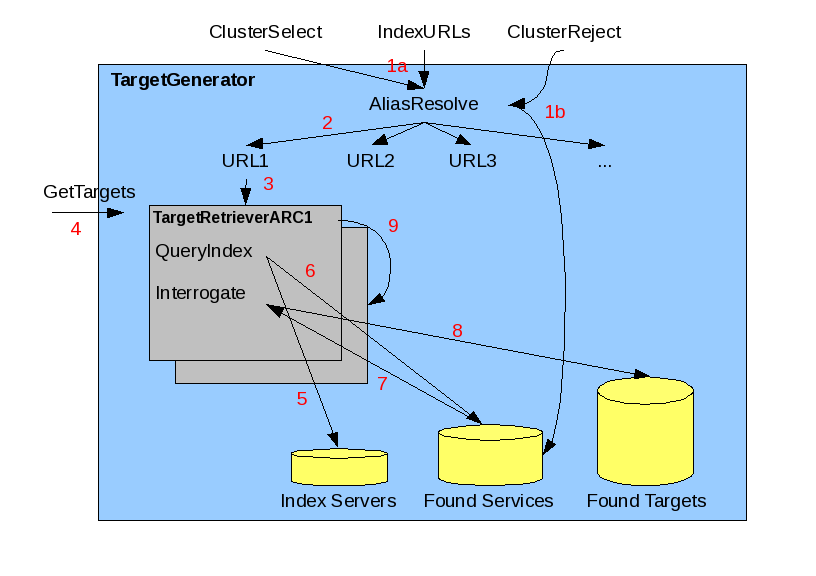
\includegraphics{TargetDiscovery.png}}}
\caption{\label{fig:ResDisc}Diagram depicting the resource discovery
  and information retrieval process}}
\end{figure}

\begin{enumerate}
\item{The {\TargetGenerator} takes three arguments as input. The first
  argument is a reference to a {\UserConfig} object containing a
  representation of the contents of the user's configuration file. The
  second and third arguments contain lists of strings. The first list
  contains individually selected and rejected computing services,
  while the second list contains individually selected and rejected
  index servers. Rejected servers and services are identified by that
  its name is prefixed by a minus sign in the lists. The name of the
  servers and services should be given either in the form of an alias
  defined in the {\UserConfig} object or as the name of its grid
  flavour followed by a colon and the URL of its information contact
  endpoint.}
\item{These lists are parsed through alias resolution before being
  used to initialize the complete list of selected and rejected
  {\URL}s pointing to computing services and index servers.}
\item{For each selected index server and computing service a
  {\TargetRetriever} plugin for the server's or service's grid flavour
  is loaded using the ARC loader. The {\TargetRetriever} is
  initialized with its {\URL} and the information about whether it
  represents a computing service or an index server.}
\item{An external call is received calling for targets to be
  prepared. The call for targets is processed by each
  {\TargetRetriever} in parallel.}
\item{A {\TargetRetriever} representing an index server first tries to
  register at the index server store kept by the {\TargetGenerator}.
  If allowed to register, the index server is queried and the query
  result processed. The {\TargetGenerator} will not allow
  registrations from index servers present in its list of rejected
  index servers or from servers that have already registered
  once. Index servers often register at more than one index server,
  thus different {\TargetRetriever}s may discover the same server.}
\item{If while processing the query result the {\TargetRetriever}
  finds an other registered index server or a registered computing
  service it creates a new {\TargetRetriever} for the found server or
  service and forwards the call for targets to the new
  {\TargetRetriever}.}
\item{A {\TargetGenerator} representing a computing service first
  tries to register at the service store kept by the
  {\TargetGenerator}. If allowed to register, the computing server is
  queried and the query result processed. The {\TargetGenerator} will
  not allow registrations from computing services present in its list
  of rejected computing services or from service that have already
  registered once. Computing services often register at more than one
  index server, thus different {\TargetRetriever}s may discover the
  same service.}
\item{When processing the query result the {\TargetRetriever} will
  create an {\ExecutionTarget} for each queue found on the computing
  service and collect all possible information about them. It will
  then store the {\ExecutionTarget} in the found targets store kept
  by the {\TargetGenerator} for later usage (e.g.\ status printing or
  job submission).}
\end{enumerate}

\section{Job Submission}
\label{sec:JobSubmission}

Job submission starts with the resource discovery and target
preparation as outlined in the Section~\ref{sec:TargetDiscovery}. Not
until a list of possible targets (which allows the user) is available
is the job description read in order to enable bulk job submission of
widely different jobs without having to reperform the resource
discovery. In addition to the classes mentioned above the job
submission makes use of the {\Broker}, {\JobDescription} and
{\Submitter} classes.  The {\Submitter} is base class for further grid
middleware specific specialization (plugin) similarly to the {\TargetRetriever}.

\begin{figure}[ht]
\centering{{\scalebox{0.75}{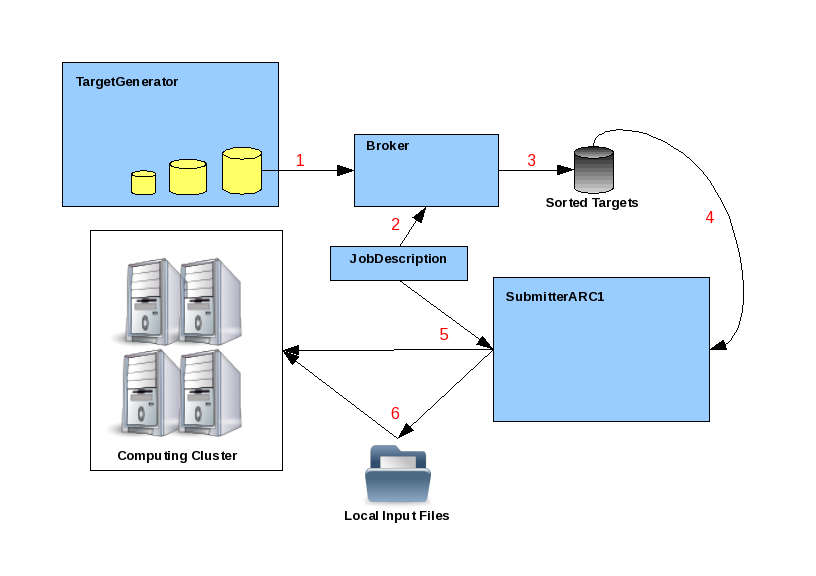
\includegraphics{JobSubmission.png}}}
\caption{\label{fig:JobSub}Diagram depicting the submission of a job
  to a computing service.}}
\end{figure}

Figure \ref{fig:JobSub} shows a job submission sequence and below a
description of each step is given:

\begin{enumerate}
\item{The {\TargetGenerator} has prepared a list of
  {\ExecutionTarget}s. Depending on the {\URL}s provided to the
  {\TargetGenerator} the list of found {\ExecutionTarget}s may be
  empty or contain several targets. Targets may even represent more
  than one grid flavour. The list of found targets are given as input
  to the {\Broker}.}
\item{In order to rank the found services ({\ExecutionTarget}s) the
  {\Broker} needs detailed knowledge about the job requirements, thus
  the {\JobDescription} is passed as input to the brokering process.}
\item{The {\Broker} filters and ranks the {\ExecutionTarget}s according 
  to the ranking method chosen by the user.}
\item{Each {\ExecutionTarget} has a method to return a specialized
  {\Submitter} which is capable of submitting jobs to the service it
  represents. The best suitable {\ExecutionTarget} for the job is
  asked to return a {\Submitter} for job submission.}
\item{The {\Submitter} takes the {\JobDescription} as input and
  uploads it to the computing service.}
\item{The {\Submitter} identifies local input files from the
  {\JobDescription} and uploads them to the computing service.}
\end{enumerate}

\section{Job Management}

Once a job is submitted job related information (job identification
string, cluster etc) is stored in a local XML file which stores this 
information for all active jobs. This file may contain jobs running on
completely different grid flavours, and thus job management should be
handled using plugins similar to resource discovery and job
submission. The job managing plugin is called the {\JobController} and
it is supported by the {\JobSupervisor} and {\Job} classes.

\begin{figure}[ht]
\centering{{\scalebox{0.75}{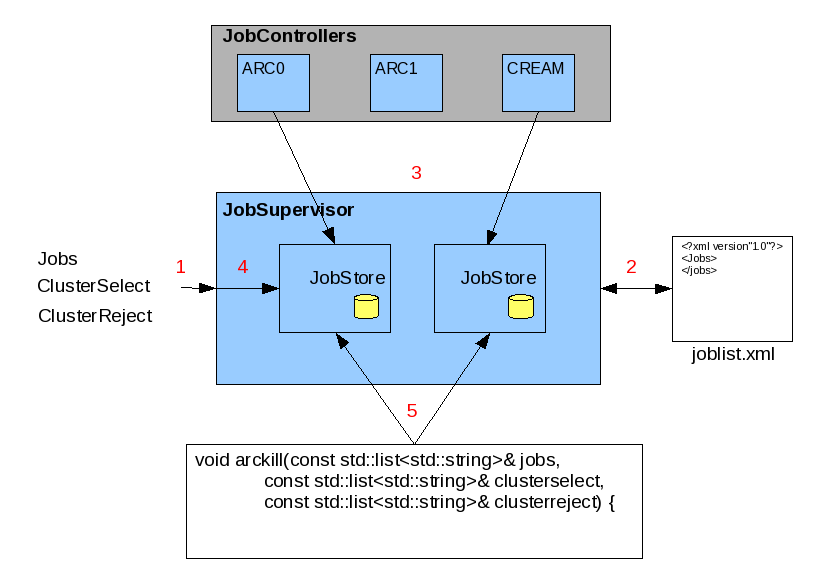
\includegraphics{JobManagement.png}}}
\caption{\label{fig:JobMan}Diagram depicting how job controlling
  plugins, {\JobController}s, are loaded and initialized.}}
\end{figure}

Figure~\ref{fig:JobMan} shows how the three different classes work
together and below a step by step description is given:

\begin{enumerate}
\item{The {\JobSupervisor} takes four arguments as input. The first
  argument is a reference to a {\UserConfig} object containing a
  representation of the contents of the user's configuration file. The
  second is a list of strings containing job identifiers and job
  names, the third is a list of strings of clusters to select or
  reject (in the same format as described for the {\TargetGenerator}
  above). The last argument is the name of the file containing the
  local information about active jobs, hereafter called the joblist
  file.}
\item{A job identifier does not uniquely define which grid flavour
  runs a certain job. Thus this information is stored in the joblist
  file upon submission by the {\Submitter} and the joblist file is
  extensively used by the {\JobSupervisor} to identify the
  {\JobController} flavours which are to be loaded. The information in
  the joblist file is also used to look up the job identifier for jobs
  specified using job names. Alias resolving for the selected and
  rejected clusters are performed using the information in the
  {\UserConfig} object.}
\item{Suitable {\JobController}s are loaded}
\item{The list of job identifiers and selected and rejected clusters
  are passed to each {\JobController} which uses the information to
  fill its internal \texttt{JobStore}.}
\item{Residing within the {\JobSupervisor} the {\JobController}s are
  now accessible for external calls (i.e. job handling).}
\end{enumerate}

\chapter{Implementation}
\label{sec:Implementation}

In this section an overview of all important classes in the new
{\libarcclient} is given. The overview is subdivided in two parts where
first all the generic classes are presented,
Section~\ref{sec:genclass}, before the grid flavour specializations
are presented in Section~\ref{sec:plugins}. Classes are described both
in words and by code.

\section{Generic Classes}
\label{sec:genclass}

\subsection{{\ACC}}

The Arc Client Component ({\ACC}) class is a base class needed for the
{\Loader} in order to create loadable classes. It stores information
about which flavour it supports and security related information
needed by all ACC specializations.

\begin{shaded}
\begin{verbatim}
class ACC {
protected:
  ACC(Config *cfg, const std::string& flavour);
public:
  virtual ~ACC();
  const std::string& Flavour();
protected:
  std::string flavour;
  std::string proxyPath;
  std::string certificatePath;
  std::string keyPath;
  std::string caCertificatesDir;
};
\end{verbatim}
\end{shaded}

\subsection{{\TargetGenerator}}

The {\TargetGenerator} class is the main class for resource discovery
and information retrieval. It loads {\TargetRetriever} plugins in
accordance with the input {\URL}s using the ARC {\Loader}~\cite{hed}
(e.g.\ if an {\URL} pointing to an ARC1 resource is given the
TargetRetrieverARC1 is loaded).

To perform a resource discovery, first construct a {\TargetGenerator}
object using the {\TargetGenerator} constructor,

\begin{shaded}
\begin{verbatim}
TargetGenerator(const UserConfig& usercfg,
                const std::list<std::string>& clusters,
                const std::list<std::string>& indexurls);
\end{verbatim}
\end{shaded}

where \texttt{clusters} and \texttt{indexurls} are lists of strings
where each string is either the name of a grid flavour followed by a
colon and the URL of an information contact endpoint for a computing
service or index server, respectively, of that grid flavour or an
alias defined in the {\UserConfig} object passed as the first
argument, e.g.:

\begin{shaded}
\begin{small}
\begin{verbatim}
ARC0:ldap://grid.tsl.uu.se:2135/Mds-Vo-name=Sweden,o=grid
ARC0:ldap://grid.tsl.uu.se:2135/nordugrid-cluster-name=grid.tsl.uu.se,Mds-Vo-name=local,o=grid
\end{verbatim}
\end{small}
\end{shaded}

where the former is the URL to an index server while the latter is an
URL to a computing service. If a string in \texttt{clusters} or
\texttt{indexurls} is prefixed by a minus sign, the corresponding
computing service or index server is rejected and excluded during
resource discovery.

To prepare a list of {\ExecutionTarget}s use the {\TargetGenerator}
object and invoke its method

\begin{shaded}
\begin{verbatim}
GetTargets(int targetType, int detailLevel);
\end{verbatim}
\end{shaded}

The {\TargetGenerator} will pass this request to the loaded
{\TargetRetriever}s running them as individual threads for improved
performance. The {\TargetGenerator} keeps records of index servers and
computing services found by the {\TargetRetriever}s in order to avoid
multiple identical queries. Accepted {\ExecutionTarget}s are stored in
the FoundTargets array kept by the {\TargetGenerator}. See also
Section~\ref{sec:TargetDiscovery} for a schematic drawing of the
resource discovery process.

Information about the found {\ExecutionTarget}s can be printed by 

\begin{shaded}
\begin{verbatim}
PrintTargetInfo(bool longlist) const;
\end{verbatim}
\end{shaded}

\subsection{{\TargetRetriever}}

The {\TargetRetriever} is base class for {\TargetRetriever} grid
middleware specializations and inherits from the {\ACC} base class in
order to be loadable by the ARC \texttt{Loader}. It is designed to
work in conjunction with the {\TargetGenerator} and contains the pure
virtual method

\begin{shaded}
\begin{verbatim}
virtual void GetTargets(TargetGenerator& mom, int targetType,
                        int detailLevel) = 0;
\end{verbatim}
\end{shaded}

which is to be implemented by the specialized class. While it is not
mandatory it is recommended that the specialized class divides this
method into two components: QueryIndex and InterrogateTarget. The
former handles index server queries, and the latter the computing
service queries and {\ExecutionTarget} preparation.

If an index server query yields a URL to a different index server
than the one queried, then the {\TargetRetriever} should call itself
recursively creating a new {\TargetRetriever} for the discovered index
server.

\subsection{{\ExecutionTarget}}

The {\ExecutionTarget} is the class representation of a computing
resource (queue) capable of executing a grid job. It serves as input
to the {\Broker} which is able to filter and rank different 
{\ExecutionTarget}s from different grid flavours without a
priori knowing their difference. The {\ExecutionTarget} class mimics
the Glue2 information model (with a flattened structure), and thus a
mapping between attributes from other information systems into the
Glue2 format is needed. Appendix \ref{app:ExTarget} shows the current
mapping for the production ARC, ARC1 and gLite middlewares.

All attributes of the {\ExecutionTarget} can be printed by the method

\begin{shaded}
\begin{verbatim}
void Print(bool longlist) const;
\end{verbatim}
\end{shaded}

Following a broker ranking jobs are to be submitted. Since all
information about the selected computing service resides within the
selected {\ExecutionTarget}, the {\ExecutionTarget} is capable of
returning a {\Submitter} capable of submitting a job to the service it
represents.

\begin{shaded}
\begin{verbatim}
Submitter *GetSubmitter(const UserConfig& ucfg) const;
\end{verbatim}
\end{shaded}

The {\UserConfig} object is used to configure the security related
information needed by the {\Submitter}.

\subsection{{\Broker}}

The {\Broker} inherits from the {\ACC} base class in order to be loadable by the ARC \texttt{Loader}. It is the base class of the 
specialized {\Broker} and it implements the method for reducing a list of resources found by resource discovery (the list of 
{\ExecutionTarget}s residing witin the {\TargetGenerator}) to a list of resources capable of running a certain job:

\begin{shaded}
\begin{verbatim}
void PreFilterTargets(Arc::TargetGenerator& targen, Arc::JobDescription jd);
\end{verbatim}
\end{shaded}

The {\texttt PreFilterTargets} method compares every hardware and software requirement given in the job description against the 
computing resource (cluster) specifications stored in the {\ExecutionTarget}. If the{\ExecutionTarget} doesn't fulfill 
the requirements imposed by the job description, or it is impossible to carry out the matchmaking due to incomplete information 
published by the computing resource, the {\ExecutionTarget} will be removed from the list of possible targets. A detailed overview 
of the matchmaking between {\JobDescription} and {\ExecutionTarget} attributes is given in Appendix~\ref{sec:broker-mapping}. 
 
Once prefiltered the remaining {\ExecutionTarget}s should be ranked in order to return the ``best'' {\ExecutionTarget} for 
job submission. Different ranking methods are implemented by the specialized brokers, but for usability and consistency reasons 
these methods are encapsulated by the {\Broker} base class method

\begin{shaded}
\begin{verbatim}
ExecutionTarget& GetBestTarget(bool &EndOfList);
\end{verbatim}
\end{shaded}

which invokes the {\texttt SortTargets} method implemented by the specialized broker (see Section~\ref{sec:brokerplugins}) 
and returns the best target. The {\texttt GetBestTarget} method is ``incremented'' at each call, thus upon a second call 
the second best {\ExecutionTarget} will be returned. 

\subsection{{\JobDescription}}

When addressing interoperability it is of paramount importance to
transparently address grid job descriptions written in different job
description languages by translating them automatically. In the
{\libarcclient} library this functionality is implemented in the
{\JobDescription} class which parses job descriptions given in the 
XRSL~\cite{xrsl}, JDL~\cite{jdl} or JSDL~\cite{jsdl} formats into an 
internal representation based upon the upcoming PGI-JSDL proposal. 

\begin{shaded}
\begin{verbatim}
bool setSource(const std::string source);
\end{verbatim}
\end{shaded}

The identification of the source description format is internally handled by a 
\texttt{JobDescriptionOrderer} class which identifies the format by pattern matching.
Once the format is determined from the elements are mapped from the original format (XRSL, JDL or JSDL) 
into the internal representation (the \texttt{JobInnerRepresentation} class). Mapping details 
are given in Section~\ref{sec:jobinnerrepresentation}. 

The {\JobDescription} class has three back-end classes, sometimes
referred to as back-end or translator modules, corresponding to the
three supported job description languages. The {\JobDescription} class
chooses the appropriate back-end module according to the pattern matching
performed by the \texttt{JobDescriptionOrderer}, and uses the back-end
module for parsing and translation (if needed) of the job descriptions.

Once the job description language required by the {\ExecutionTarget} chosen 
for job submission is known the parsed and (if needed) translated job description 
can be retrieved through the {\texttt GetProduct} funcion as shown below:

\begin{shaded}
\begin{verbatim}
bool getProduct(std::string& product, std::string format = "POSIXJSDL")
\end{verbatim}
\end{shaded}

If the inner representation is empty or the source job descrition is not
valid, then the {\texttt GetProduct} output is empty too and the method 
returns with false. When the product format is the same as the source format 
and not XRSL, than the product string is set to the source string. The XRSL 
output is always generated from the inner representation, as it includes 
automatic job description modifications similar to those of the production 
ARC client. If the product format differs from the source format the 
{\texttt GetProduct} method calls upon the \texttt{JobDescriptionOrderer} 
class to carry out the translation.

The translation of a job description basically means a syntactical transformation 
of the job description from one language to another. Thus the {\JobDescription}
class can do nothing in those cases where there is not enough data is available 
to assemble a given attribute or when information can be lost because the received 
attribute has no equivalent in the output language. In these events the {\texttt GetProduct} 
method returns with a false and an empty product stringt. For limitations in the translation
see Section~\ref{sec:jobinnerrepresentation}.

For the JSDL output generation the {\JobDescription} class uses
the core JSDL's capabilities amended with the JSDL-POSIX and JSDL-ARC
extensions. The loss of information is minimal in case of generating
such an output.

For the JDL generation the latest version of JDL specification was
used (v0.9) \cite{jdl}. Deprecated and backward compatibility
attributes are not implemented.

\subsection{{\Submitter}}

{\Submitter} is base class for grid specific specializations (plugin).
It submits job(s) to the service it represents and uploads (by the job
needed) local input files.

\begin{shaded}
\begin{verbatim}
virtual bool Submit(JobDescription& jobdesc, XMLNode& info) = 0;
\end{verbatim}
\end{shaded}

The \texttt{Submit} method fills the {\XMLNode} \texttt{info} with all
needed information about the job for later job management. The
{\Submitter} is returned by the {\ExecutionTarget} selected for job
execution and thus the {\ExecutionTarget} populates (through its
{\XMLNode} config element) the {\Submitter} with information about
submission endpoint ({\URL}) and job description languages understood
by the target.

\subsection{{\JobSupervisor}}

The {\JobSupervisor} is responsible for loading the appropriate
{\JobController}s for managing jobs running on a certain grid
flavour. Job manipulation can be performed either on individual jobs
or on groups of jobs (e.g.\ all jobs running on certain cluster or all
jobs with job state ``FINISHED''), and in order to translate the
information given by the user into a set of loadable {\JobController}s
the {\JobSupervisor} makes extensive use of the local joblist file
housing information about all active jobs. Thus the {\JobSupervisor}
constructor becomes

\begin{shaded}
\begin{verbatim}
JobSupervisor(const UserConfig& usercfg,
              const std::list<std::string>& jobs,
              const std::list<std::string>& clusters,
              const std::string& joblist);
\end{verbatim}
\end{shaded}

where \texttt{jobs} is a list of job identifiers and job names,
\texttt{clusters} is a list of selected and rejected computing
services in the same format as described above for the
{\TargetGenerator}, \texttt{joblist} is a string containing the name
of the joblist file.

Although being loaded by the {\JobSupervisor} the {\JobController}
objects truly resides within the ARC {\Loader} which is a member of
the {\JobSupervisor} class. In order to get handles on the
{\JobController}s the inline method

\begin{shaded}
\begin{verbatim}
const std::list<Arc::JobController*>& GetJobControllers();
\end{verbatim}
\end{shaded}

returns a list of pointers to the loaded {\JobController}s.

\subsection{{\JobController}}

The {\JobController} is a base class for grid specific
specializations, but also the implementer of all public functionality
offered by the {\JobController}s. In other words all virtual functions
of the {\JobController} are private. The initialization of a
(specialized) {\JobController} object takes two steps. First the
{\JobController} specialization for the required grid flavour must be
loaded by the ARC {\Loader}, which sees to that the {\JobController}
receives information about its flavour (grid) and the local joblist
file containing information about all active jobs (flavour
independent). Next step is the filling of the {\JobController}'s job
pool \texttt{JobStore} which is the pool of jobs that the
{\JobController} can manage.

\begin{shaded}
\begin{verbatim}
void FillJobStore(const std::list<URL>& jobids,
                  const std::list<URL>& clusterselect,
                  const std::list<URL>& cluterreject);
\end{verbatim}
\end{shaded}

Here \texttt{jobids}, \texttt{clusterselect} and
\texttt{clusterreject} have been resolved for job names and aliases by
the {\JobSupervisor}, and no further resolution is needed. The
following rules are observed when filling the \texttt{JobStore}:

\begin{enumerate}
\item{If the \texttt{jobids} list has entries, fill \texttt{JobStore}
  with the by user requested jobs.}
\item{If the \texttt{clusterselect} list has entries, fill
  \texttt{JobStore} with the jobs running on the selected clusters.}
\item{If clusters are rejected and \texttt{JobStore} has entries,
  remove from \texttt{JobStore} all jobs running on rejected
  clusters.}
\item{If \texttt{jobs} and \texttt{clusterselect} are both empty
  lists, fill \texttt{JobStore} with all jobs except those running on
  possible rejected clusters.}
\end{enumerate}

The steps above completes the initialization of the {\JobController}
which is now ready for handling jobs. The public functions of the
{\JobController} offer to get (download), clean, cancel, etc one or
more jobs and uses the private specializations for issuing the
command. Here exemplified by the \texttt{Stat} command:

\begin{shaded}
\begin{small}
\begin{verbatim}
bool JobController::Stat(const std::list<std::string>& status,
                         const bool longlist,
                         const int timeout) {

  GetJobInformation();

  for (std::list<Job>::iterator it = jobstore.begin();
       it != jobstore.end(); it++) {
    if (it->State.empty()) {
      logger.msg(WARNING, "Job state information not found: %s",
                 it->JobID.str());
      Time now;
      if (now - it->LocalSubmissionTime < 90)
        logger.msg(WARNING, "This job was very recently "
                   "submitted and might not yet"
                   "have reached the information-system");
      continue;
    }
    it->Print(longlist);
  }
  return true;
}
\end{verbatim}
\end{small}
\end{shaded}

The \texttt{Stat} command prints the job information to screen and in
order to do so the {\JobController} has to query local information
server for the latest status. Due to different protocols used for
different grid flavours (e.g.\ ldap for production ARC), the
\texttt{GetJobInformation} has to be grid flavour specific and is only
declared as a private virtual method within the {\JobController} base
class. For details about the flavour specific implementations see
Section~\ref{sec:plugins}.

\subsection{{\Job}}

The {\Job} is a generic job class for storing all job related
information. Attributes are derived from the Glue2 information model
and thus a mapping is needed for non Glue2 compliant grid middlewares.
Appendix~\ref{app:job} shows the present mapping schema.

All attributes of the {\Job} can be printed by the method

\begin{shaded}
\begin{verbatim}
void Print(bool longlist) const;
\end{verbatim}
\end{shaded}

\subsection{{\UserConfig}}

The {\UserConfig} class handles the client setup i.e. proxy,
certificate and key location, user and system configuration and local
joblist location. Upon initialization (constructor) the {\UserConfig}
locates the user files

\begin{shaded}
\begin{verbatim}
$HOME/.arc/client.xml
$HOME/.arc/jobs.xml
\end{verbatim}
\end{shaded}

and if either of them is non-existing a default (empty) one is created.

The {\UserConfig} has three main public methods

\begin{shaded}
\begin{verbatim}
const std::string& JobListFile() const;
const XMLNode& ConfTree() const;
bool ApplySecurity(XMLNode& ccfg) const;
\end{verbatim}
\end{shaded}

where \texttt{JobListFile()} returns the string pointing to the
jobs.xml file while \texttt{ConfTree()} returns a configuration
{\XMLNode} object which is the merge between the user and system
configurations. In order to do this the method has to locate the
system configuration and resolve possible conflicts with the user
configuration. This proceeds through the following chain of actions:

\begin{enumerate}
\item{Try reading system configuration from \texttt{<ARC Install
    Location>/etc/arcclient.xml}}
\item{If the previous step failed try reading system configuration
  from \texttt{/etc/arcclient.xml}}
\item{Merge system and user configuration by adding all system
  configuration not already listed in the user configuration to the
  latter.}
\end{enumerate}

The \texttt{ApplySecurity(XMLNode\& ccfg)} adds security tags to the
ccfg {\XMLNode} as follows:

\begin{itemize}
\item{If the \texttt{\$X509\_USER\_PROXY} environment variable is set,
  use its value to define a \texttt{ProxyPath} tag in \texttt{cfg}. If
  the file does not exist or can't be read exit with an error.}
\item{Otherwise, if the \texttt{\$X509\_USER\_CERT} environment
  variable is set, use its value and the value of the
  \texttt{\$X509\_USER\_KEY} environment variable to define
  \texttt{CertificatePath} and \texttt{KeyPath} tags in \texttt{cfg}.
  If \texttt{\$X509\_USER\_KEY} is not set or either file does not
  exist or can't be read exit with an error.}
\item{Otherwise, if the merged user configuration tree (see
  \texttt{ConfTree} contains a \texttt{ProxyPath} tag, copy it to
  \texttt{cfg}. If the file does not exist or can't be read exit with
  an error.}
\item{Otherwise, if the merged user configuration tree contains a
  \texttt{CertificatePath} tag, copy it to \texttt{cfg} along with the
  accompanying \texttt{KeyPath} tag. If the \texttt{KeyPath} tag is
  undefined or either file does not exist or can't be read exit with
  an error.}
\item{Otherwise, if the file \texttt{/tmp/x509up\_u + userid} exists
  add a \texttt{ProxyPath} tag in \texttt{cfg} pointing to it.}
\item{Otherwise, add \texttt{CertificatePath} and \texttt{KeyPath}
  tags to \texttt{cfg} pointing to
  \texttt{\$HOME/.globus/usercert.pem} and
  \texttt{\$HOME/.globus/userkey.pem}, respectively. If either file
  does not exist exit with error.}
\item{If the \texttt{\$X509\_CERT\_DIR} environment variable is set,
  use its value to define a \texttt{CACertificatesDir} tag in
  \texttt{cfg}. If the directory does not exist, exit with an error.}
\item{Otherwise, if the user ID is not zero and the directory
  \texttt{\$HOME/.globus/certificates} exists add a
  \texttt{CACertificatesDir} tag in \texttt{cfg} pointing to it.}
\item{Otherwise, add a \texttt{CACertificatesDir} tag in \texttt{cfg}
  pointing to \texttt{/etc/grid-security/certificates}. If the
  directory does not exist, exit with an error.}
\end{itemize}

\subsection{{\ACCConfig}}

Locating Arc Client Components (plugins) is handled by the
{\ACCConfig} class. It inherits from \texttt{BaseConfig} and
implements only one method

\begin{shaded}
\begin{verbatim}
virtual XMLNode MakeConfig(XMLNode cfg) const;
\end{verbatim}
\end{shaded}

The \texttt{MakeConfig} method searches plugin paths for all libraries
named \texttt{libacc*}. Matching libraries are added as plugins to the
configuration object \texttt{cfg}.

\subsection{{\ClientInterface}}

The {\ClientInterface} class is a utility base class used for
configuring a client side Message Chain Component (MCC) chain and
loading it into memory. It has several specializations of increasing
complexity of the MCC chains.

\subsubsection{{\ClientTCP}}

The {\ClientTCP} class is a specialization of the {\ClientInterface}
which sets up a client MCC chain for TCP communication, and optionally
with a TLS layer on top.

\subsubsection{{\ClientHTTP}}

The {\ClientHTTP} class inherits from the {\ClientTCP} class and adds
an HTTP MCC to the chain.

\subsubsection{{\ClientSOAP}}

The {\ClientSOAP} class inherits from the {\ClientHTTP} class and adds
a SOAP MCC to the chain. Specializations of the {\TargetRetriever},
{\Submitter} and {\JobController} classes that communicate with SOAP
based services make use of this class.

\section{Specialized Classes (Grid Flavour and Broker plugins)}
\label{sec:plugins}

\subsection{ARC0 Plugins}

The ARC0 plugins enables support for the interfaces used by computing
elements running ARC version 0.x.

The ARC 0.x local information system uses the {\GT}~\cite{globus} GRIS
with a purpose made ARC schema. The information index server used is the
{\GT} GIIS. Both these servers are using the LDAP~\cite{ldap}
protocol. The specialization of the {\TargetRetriever} class for ARC0
is implemented using the ARC LDAP Data Management Component (DMC) (see
\cite{hed} for technical details).

Jobs running on an ARC 0.x computing element are handled by the ARC
grid-manager~\cite{gm}. Job submission and job control are done using
the gridftp~\cite{gridftp} protocol. The specializations of the
{\Submitter} and {\JobController} classes use the globus ftp control
library.

Stage-in and stage-out of input and output files are also done using
the gridftp~\cite{gridftp} protocol. This means that proper
functionality of the ARC0 plugins requires the gridftp DMC.

\subsection{ARC1 Plugins}

The computing element in ARC version 1.x is the A-Rex~\cite{arex}
service running in a HED~\cite{hed} container.

A-Rex implements the BES~\cite{ogsa-bes} standard interface. Since
this is a SOAP~\cite{soap} based interface the specializations of the
{\TargetRetriever}, {\Submitter} and {\JobController} classes make use
of a chain of ARC Message Chain Components (MCC~\cite{hed}) ending
with the SOAP client MCC.

The A-Rex service uses the https protocol put and get methods for
stage-in and stage-out of input and output files. Therefore, the ARC1
plugins requires the http DMC.

\subsection{gLite Plugins}

The gLite computing element offers several interfaces, one of them
being the Web Service based computing element interface known as the
CREAM CE~\cite{cream}. The current revision of this interface (CREAM
version 2) has been chosen for implementation within {\libarcclient} for the
following reasons:

\begin{itemize}
\item CREAM2 has a Web Service interface that fits the Web Service
  based ARC.
\item CREAM2 enables direct access to the gLite computing element
  without having to go via the gLite workload management system.
\item CREAM2 contains numerous improvements when compared to the
  earlier CREAM versions.
\item CREAM2 supports direct job status queries.
\item CREAM2 offers a convenient way of handling input and output
  files through accessing the input and output sandbox via GridFTP.
\end{itemize}

gLite resources are registered in top level and site BDIIs. The CREAM
specialization of the {\TargetRetriever} therefore makes use of the
LDAP DMC similarly to the ARC0 plugins.

CREAM has its own SOAP based interface. The CREAM
specializations of the {\Submitter} and {\JobController} classes
therefore use an MCC chain ending with the SOAP client MCC the same 
way the ARC1 plugin does.

Stage-in and stage-out of input and output files are done using the
gridftp protocol. The gridftp DMC is therefore required.

\subsection{Broker plugins}
\label{sec:brokerplugins}

\subsubsection{\RandomBroker}

The {\RandomBroker} ranks the {\ExecutionTarget}s randomly. 

\subsubsection{\FastestCPUBroker}

The {\FastestCPUBroker} ranks the {\ExecutionTarget}s according to their CPU performance. The most 
reliable comparison is achieved through the usage of a benchmark scenario, and the {\FastestCPUBroker}
uses the CINT2000 (Integer Component of SPEC CPU2000)\footnote{http://www.spec.org/cpu2000/CINT2000/} 
benchmark for this purpose. 

The {\texttt SortTargets} method has two steps:

\begin{enumerate}
\item{{\ExecutionTarget}s not publishing the specint2000 benchmark information are removed from the list 
  of possible targets as their performance is unknown.}
\item{The {\ExecutionTarget}s are ranked such that the {\ExecutionTarget} with highest specint2000 value 
  receives top ranking}
\end{enumerate}

\subsubsection{\FastestQueueBroker}

The {\FastestQueueBroker} ranks the {\ExecutionTarget}s according to their queue length measured in percentage 
of the {\ExecutionTarget}'s size (i.e. the queue length divided by the number of total slots/CPUs). If more 
than one {\ExecutionTarget} has zero queue, the {\FastestQueueBroker} makes use of a basic load balancing method 
to rearrange the zero queue {\ExecutionTarget}s depending on their number of free slots/CPUs. 

The {\texttt SortTargets} method has three steps:

\begin{enumerate}
\item{{\ExecutionTarget}s not publishing WaitingJobs, TotalSlots and FreeSlots are removed from the list of possible targets 
as it is impossible to determine their queue length and perform load balancing.}
\item{The {\ExecutionTarget}s are ranked according to their queue length relative to the number of slots/CPUs. Zero queue 
{\ExecutionTarget}s is ranked top.}
\item{If more than one {\ExecutionTarget} has zero queue the targets are randomly reshuffled based upon how many free slots 
they have. E.g. if two {\ExecutionTarget}s have zero queue and they have 90 and 10 free slots respectively, then the first
{\ExecutionTarget} has a 90\% propability of becoming the top ranked cluster.}
\end{enumerate}

\subsubsection{\DataBroker}

The {\DataBroker} ranks the {\ExecutionTarget}s according to how many megabytes of the requested input files that already 
stored in the cache of the computing resource the {\ExecutionTarget} represents. The broker is motivated by that jobs should 
be submitted to {\ExecutionTarget}s where the data already is, thus reducing the network load on both the computing resource 
and client side. The ranking method is based upon the A-REX\footnote{http://www.knowarc.eu/download/D1.2-3\_documentation.pdf} 
interface {\texttt CacheCheck} for querying for the presence of the file in the cache directory. This interface has a limitation 
in the current implementation as it can only use cache directory of format

\begin{shaded}
\begin{verbatim}
cachedir="/tmp/cache"
\end{verbatim}
\end{shaded}

If the cachedir parameter involves {\%}U or other substitute element then the {\texttt CacheCheck} will not work.

The {\texttt SortTargets} method has four steps:

\begin{enumerate}
\item{Only the A-REX service has {\texttt CacheCheck} method, thus {\ExecutionTarget}s not running A-REX are removed.
therefore the other clusters will be ignored.}
\item{Information about input files is collected from the JobInnerRepresentation.}
\item{Each {\ExecutionTarget} is queried (through the {\texttt CacheCheck} method) for the existence of input files. 
A single query is used for achieving all the necessary information and file sizes are summarized. If there is problems 
determining file sizes, then the summarized size will be zero.}
\item{The possible {\ExecutionTarget}s are ranked in a descending order according to the amount of input data they have in cache.}
\end{enumerate}

Example of a CacheCheck request that can be sent to an A-REX service:

\begin{shaded}
\begin{verbatim}
<CacheCheck>
   <TheseFilesNeedToCheck>
       <FileURL>http://knowarc1.grid.niif.hu/storage/Makefile</FileURL>
       <FileURL>ftp://download.nordugrid.org/test/README</FileURL>
   </TheseFilesNeedToCheck>
</CacheCheck>
\end{verbatim}
\end{shaded}

Example CacheCheck response from the A-REX service:

\begin{shaded}
\begin{verbatim}
<CacheCheckResponse>
   <CacheCheckResult>
   <Result>
         <FileURL>http://knowarc1.grid.niif.hu/storage/Makefile</FileURL>
         <ExistInTheCache>true</ExistInTheCache>
         <FileSize>30</FileSize>
   </Result>
   <Result>
         <FileURL>http://knowarc1.grid.niif.hu/storage/Makefile</FileURL>
         <ExistInTheCache>true</ExistInTheCache>
         <FileSize>30</FileSize>
   </Result>
  </CacheCheckResult>
</CacheCheckResponse>
\end{verbatim}
\end{shaded}
   
\subsubsection{\PythonBroker}

This {\PythonBroker} allows users to write their customized broker in
python. To use this broker the user should write a python class which 
should contain:

\begin{itemize}

\item{an \_\_init\_\_ method that takes a Config object as input, and}
\item{a SortTargets method that takes a python list of ExecutionTarget
  objects and a JobInnerRepresentation object as input.}

\end{itemize}

The {\Config}, {\ExecutionTarget} and {\texttt JobInnerRepresentation} classes are
available in the swig generated arc python module.

To invoke the {\PythonBroker}, the name of the python module defining
the broker class and the name of the broker class must be given. If
e.g. the broker class MyBroker is defined in the python module
SampleBroker the command line option to arcsub to use this broker is:

\begin{shaded}
\begin{verbatim}
-b PythonBroker:SampleBroker.MyBroker
\end{verbatim}
\end{shaded}

Additional arguments to the python broker can be added by appending
them after an additional colon after the python class name:

\begin{shaded}
\begin{verbatim}
-b PythonBroker:SampleBroker.MyBroker:args
\end{verbatim}
\end{shaded}

Extracting these additional arguments should be done in the python
broker class's \_\_init\_\_ method.

For a complete example of a simple python broker see the
SampleBroker.py file that comes with your arc python installation.

\chapter{Building Command Line Interfaces}
\label{sec:cli}

Given all components listed above it is possible to write versatile
command line interfaces (cli) for grid job submission and
management. {\libarcclient} offers the following native commands:

\begin{enumerate}
\item{\texttt{arcstat} - for computing resource or grid job status
  queries.}
\item{\texttt{arcsub} - for grid job submission}
\item{\texttt{arcget} - for downloading output of finished, cancelled
  or failed grid jobs.}
\item{\texttt{arckill} - for terminating grid jobs.}
\item{\texttt{arcclean} - for removing a grid job's session directory
  including all contents}
\item{\texttt{arccat} - for performing the \texttt{cat} command to a
  running grid job's std out or std error file.}
\end{enumerate}

Each of the commands above are encoded within one C++ file with the
following structure, here exemplified with the arcget command:

\begin{shaded}
\begin{verbatim}
#ifdef HAVE_CONFIG_H
#include <config.h>
#endif

#include <iostream>
#include <list>
#include <string>

#include <arc/ArcLocation.h>
#include <arc/IString.h>
#include <arc/Logger.h>
#include <arc/OptionParser.h>
#include <arc/client/JobController.h>
#include <arc/client/JobSupervisor.h>
#include <arc/client/UserConfig.h>

int main(int argc, char **argv) {

  setlocale(LC_ALL, "");

  Arc::Logger logger(Arc::Logger::getRootLogger(), "arcget");
  Arc::LogStream logcerr(std::cerr);
  Arc::Logger::getRootLogger().addDestination(logcerr);
  Arc::Logger::getRootLogger().setThreshold(Arc::WARNING);

  Arc::ArcLocation::Init(argv[0]);

  Arc::OptionParser options(istring("[job ...]"),
                            istring("The arcget command is used for "
                                    "retrieving the results from a job."),
                            istring("Argument to -c has the format "
                                    "Flavour:URL e.g.\n"
                                    "ARC0:ldap://grid.tsl.uu.se:2135/"
                                    "nordugrid-cluster-name=grid.tsl.uu.se,"
                                    "Mds-Vo-name=local,o=grid"));

  bool all = false;
  options.AddOption('a', "all",
                    istring("all jobs"),
                    all);

  // Removed most of the option definition from this write-up to
  // save space. See the real source file for the complete list.
  // ...

  bool version = false;
  options.AddOption('v', "version", istring("print version information"),
                    version);

  std::list<std::string> jobs = options.Parse(argc, argv);

  if (!debug.empty())
    Arc::Logger::getRootLogger().setThreshold(Arc::string_to_level(debug));

  Arc::UserConfig usercfg(conffile);
  if (!usercfg) {
    logger.msg(Arc::ERROR, "Failed configuration initialization");
    return 1;
  }

  if (debug.empty() && usercfg.ConfTree()["Debug"]) {
    debug = (std::string)usercfg.ConfTree()["Debug"];
    Arc::Logger::getRootLogger().setThreshold(Arc::string_to_level(debug));
  }

  if (version) {
    std::cout << Arc::IString("%s version %s", "arcget", VERSION)
              << std::endl;
    return 0;
  }

  if (jobs.empty() && joblist.empty() && !all) {
    logger.msg(Arc::ERROR, "No jobs given");
    return 1;
  }

  if (joblist.empty())
    joblist = usercfg.JobListFile();

  Arc::JobSupervisor jobmaster(usercfg, jobs, clusters, joblist);

  std::list<Arc::JobController*> jobcont = jobmaster.GetJobControllers();

  if (jobcont.empty()) {
    logger.msg(Arc::ERROR, "No job controllers loaded");
    return 1;
  }

  int retval = 0;
  for (std::list<Arc::JobController*>::iterator it = jobcont.begin();
       it != jobcont.end(); it++)
    if (!(*it)->Get(status, downloaddir, keep, timeout))
      retval = 1;

  return retval;
}
\end{verbatim}
\end{shaded}

\appendix

\chapter{{\ExecutionTarget}}
\label{app:ExTarget}

http://svn.nordugrid.org/trac/nordugrid/browser/arc1/trunk/doc/client/ExecutionTargetMapping.html

\chapter{Broker mapping}
\label{app:broker-mapping}

http://svn.nordugrid.org/trac/nordugrid/browser/arc1/trunk/doc/client/broker-mapping.ods

\chapter{Job Inner Representation}
\label{app:jobinnerrepresentation}

http://svn.nordugrid.org/trac/nordugrid/browser/arc1/trunk/doc/client/JobInnerRepresentation.ods

\bibliography{grid}

\end{document}
